\documentclass{standalone}
\usepackage{tikz}
\usetikzlibrary{patterns, positioning}

\begin{document}
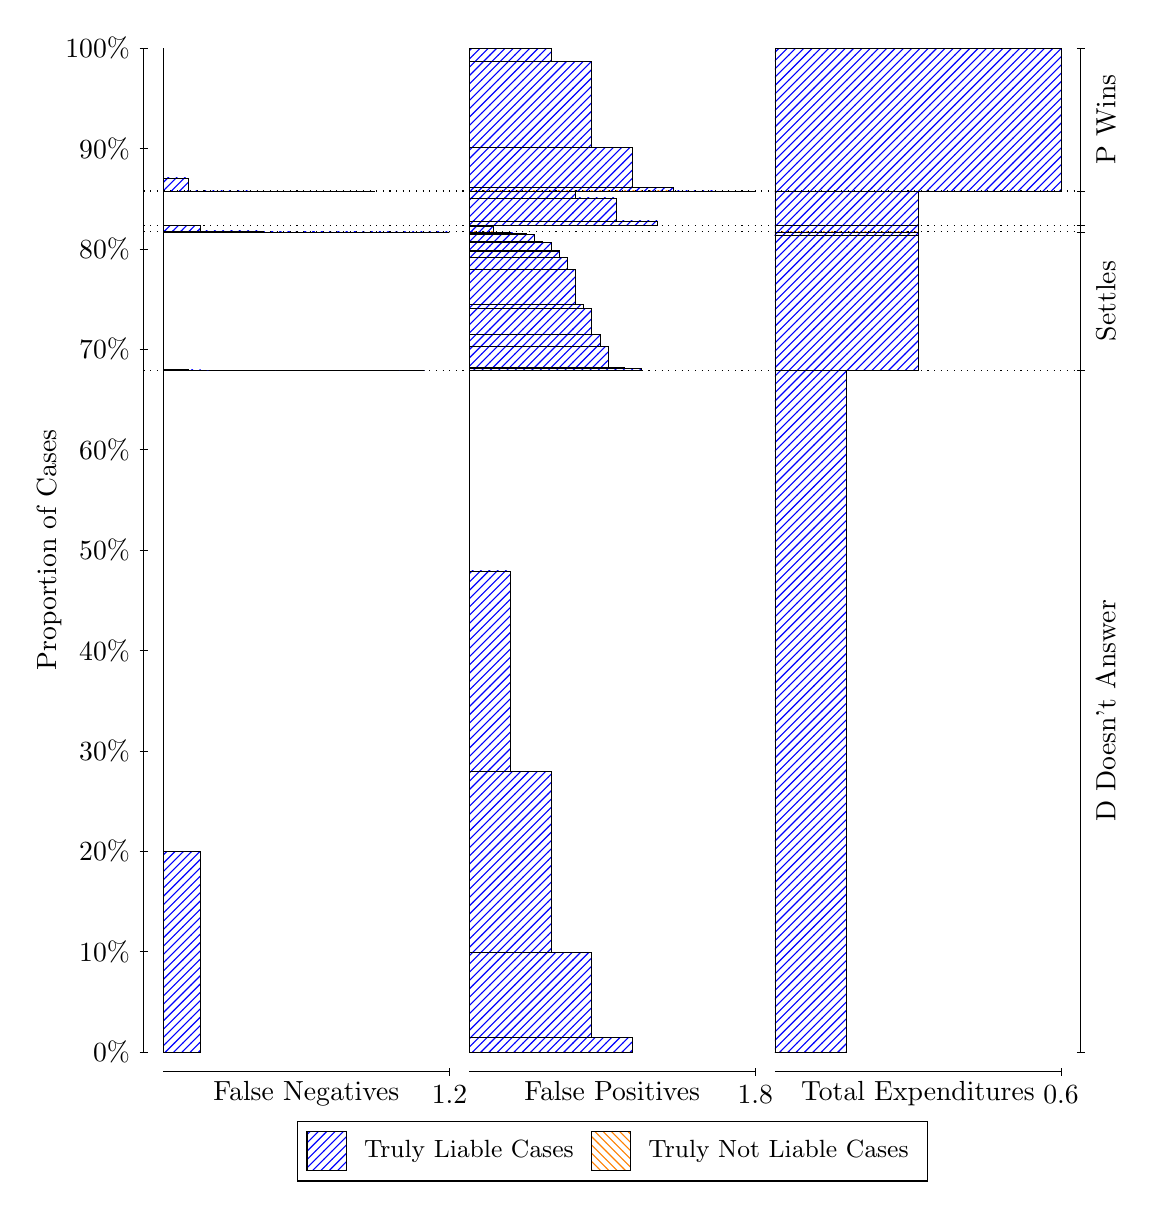
\begin{tikzpicture}
\draw[black, very thin] (1.5,1.75) -- (1.5,14.5);
\node[rotate=90, anchor=center] at (0.3, 8.125) {Proportion of Cases};
\draw[black, very thin] (1.45,1.75) -- (1.55,1.75);
\node[anchor=east] at (1.45, 1.75) {0\%};
\draw[black, very thin] (1.45,3.025) -- (1.55,3.025);
\node[anchor=east] at (1.45, 3.025) {10\%};
\draw[black, very thin] (1.45,4.3) -- (1.55,4.3);
\node[anchor=east] at (1.45, 4.3) {20\%};
\draw[black, very thin] (1.45,5.575) -- (1.55,5.575);
\node[anchor=east] at (1.45, 5.575) {30\%};
\draw[black, very thin] (1.45,6.85) -- (1.55,6.85);
\node[anchor=east] at (1.45, 6.85) {40\%};
\draw[black, very thin] (1.45,8.125) -- (1.55,8.125);
\node[anchor=east] at (1.45, 8.125) {50\%};
\draw[black, very thin] (1.45,9.4) -- (1.55,9.4);
\node[anchor=east] at (1.45, 9.4) {60\%};
\draw[black, very thin] (1.45,10.675) -- (1.55,10.675);
\node[anchor=east] at (1.45, 10.675) {70\%};
\draw[black, very thin] (1.45,11.95) -- (1.55,11.95);
\node[anchor=east] at (1.45, 11.95) {80\%};
\draw[black, very thin] (1.45,13.225) -- (1.55,13.225);
\node[anchor=east] at (1.45, 13.225) {90\%};
\draw[black, very thin] (1.45,14.5) -- (1.55,14.5);
\node[anchor=east] at (1.45, 14.5) {100\%};

\draw[black, very thin] (13.4,1.75) -- (13.4,14.5);
\draw[black, very thin] (13.35,1.75) -- (13.45,1.75);
\node[anchor=west] at (13.35, 1.75) {};
\draw[black, very thin] (13.35,10.41) -- (13.45,10.41);
\node[anchor=west] at (13.35, 10.41) {};
\draw[black, very thin] (13.35,12.166) -- (13.45,12.166);
\node[anchor=west] at (13.35, 12.166) {};
\draw[black, very thin] (13.35,12.251) -- (13.45,12.251);
\node[anchor=west] at (13.35, 12.251) {};
\draw[black, very thin] (13.35,12.684) -- (13.45,12.684);
\node[anchor=west] at (13.35, 12.684) {};
\draw[black, very thin] (13.35,14.5) -- (13.45,14.5);
\node[anchor=west] at (13.35, 14.5) {};

\draw[black, very thin, pattern color=blue, pattern=north east lines] (1.75,1.75) rectangle (2.2239,4.2999);
\draw[black, very thin, pattern color=orange, pattern=north west lines] (1.75,4.2999) rectangle (1.75,4.2999);
\draw[black, very thin, pattern color=blue, pattern=north east lines] (1.75,4.2999) rectangle (1.75,10.41);
\draw[black, very thin, pattern color=blue, pattern=north east lines] (1.75,10.41) rectangle (5.0674,10.41);
\draw[black, very thin, pattern color=blue, pattern=north east lines] (1.75,10.41) rectangle (4.7514,10.41);
\draw[black, very thin, pattern color=blue, pattern=north east lines] (1.75,10.41) rectangle (4.4355,10.41);
\draw[black, very thin, pattern color=blue, pattern=north east lines] (1.75,10.41) rectangle (4.2775,10.41);
\draw[black, very thin, pattern color=blue, pattern=north east lines] (1.75,10.41) rectangle (4.1196,10.41);
\draw[black, very thin, pattern color=blue, pattern=north east lines] (1.75,10.41) rectangle (3.9616,10.41);
\draw[black, very thin, pattern color=blue, pattern=north east lines] (1.75,10.41) rectangle (3.8036,10.41);
\draw[black, very thin, pattern color=blue, pattern=north east lines] (1.75,10.41) rectangle (3.6457,10.41);
\draw[black, very thin, pattern color=blue, pattern=north east lines] (1.75,10.41) rectangle (3.4877,10.41);
\draw[black, very thin, pattern color=blue, pattern=north east lines] (1.75,10.41) rectangle (3.3297,10.41);
\draw[black, very thin, pattern color=blue, pattern=north east lines] (1.75,10.41) rectangle (3.1717,10.41);
\draw[black, very thin, pattern color=blue, pattern=north east lines] (1.75,10.41) rectangle (3.1717,10.41);
\draw[black, very thin, pattern color=blue, pattern=north east lines] (1.75,10.41) rectangle (3.0138,10.41);
\draw[black, very thin, pattern color=blue, pattern=north east lines] (1.75,10.41) rectangle (2.8558,10.41);
\draw[black, very thin, pattern color=blue, pattern=north east lines] (1.75,10.41) rectangle (2.6978,10.41);
\draw[black, very thin, pattern color=blue, pattern=north east lines] (1.75,10.41) rectangle (2.6978,10.41);
\draw[black, very thin, pattern color=blue, pattern=north east lines] (1.75,10.41) rectangle (2.5399,10.411);
\draw[black, very thin, pattern color=blue, pattern=north east lines] (1.75,10.411) rectangle (2.3819,10.411);
\draw[black, very thin, pattern color=blue, pattern=north east lines] (1.75,10.411) rectangle (2.3819,10.411);
\draw[black, very thin, pattern color=blue, pattern=north east lines] (1.75,10.411) rectangle (2.2239,10.413);
\draw[black, very thin, pattern color=blue, pattern=north east lines] (1.75,10.413) rectangle (2.0659,10.416);
\draw[black, very thin, pattern color=blue, pattern=north east lines] (1.75,10.416) rectangle (2.0659,10.416);
\draw[black, very thin, pattern color=blue, pattern=north east lines] (1.75,10.416) rectangle (1.908,10.419);
\draw[black, very thin, pattern color=blue, pattern=north east lines] (1.75,10.419) rectangle (1.908,10.422);
\draw[black, very thin, pattern color=blue, pattern=north east lines] (1.75,10.422) rectangle (1.75,10.425);
\draw[black, very thin, pattern color=orange, pattern=north west lines] (1.75,10.425) rectangle (1.75,10.425);
\draw[black, very thin, pattern color=blue, pattern=north east lines] (1.75,10.425) rectangle (1.75,12.166);
\draw[black, very thin, pattern color=blue, pattern=north east lines] (1.75,12.166) rectangle (5.3833,12.166);
\draw[black, very thin, pattern color=blue, pattern=north east lines] (1.75,12.166) rectangle (4.5935,12.166);
\draw[black, very thin, pattern color=blue, pattern=north east lines] (1.75,12.166) rectangle (3.8036,12.166);
\draw[black, very thin, pattern color=blue, pattern=north east lines] (1.75,12.166) rectangle (3.0138,12.178);
\draw[black, very thin, pattern color=blue, pattern=north east lines] (1.75,12.178) rectangle (2.2239,12.251);
\draw[black, very thin, pattern color=orange, pattern=north west lines] (1.75,12.251) rectangle (1.75,12.251);
\draw[black, very thin, pattern color=blue, pattern=north east lines] (1.75,12.251) rectangle (2.2239,12.251);
\draw[black, very thin, pattern color=orange, pattern=north west lines] (1.75,12.251) rectangle (1.75,12.251);
\draw[black, very thin, pattern color=blue, pattern=north east lines] (1.75,12.251) rectangle (1.75,12.684);
\draw[black, very thin, pattern color=blue, pattern=north east lines] (1.75,12.684) rectangle (4.4355,12.684);
\draw[black, very thin, pattern color=blue, pattern=north east lines] (1.75,12.684) rectangle (3.6457,12.684);
\draw[black, very thin, pattern color=blue, pattern=north east lines] (1.75,12.684) rectangle (2.8558,12.684);
\draw[black, very thin, pattern color=blue, pattern=north east lines] (1.75,12.684) rectangle (2.8558,12.686);
\draw[black, very thin, pattern color=blue, pattern=north east lines] (1.75,12.686) rectangle (2.0659,12.687);
\draw[black, very thin, pattern color=blue, pattern=north east lines] (1.75,12.687) rectangle (2.0659,12.852);
\draw[black, very thin, pattern color=orange, pattern=north west lines] (1.75,12.852) rectangle (1.75,12.852);
\draw[black, very thin, pattern color=blue, pattern=north east lines] (1.75,12.852) rectangle (1.75,14.5);
\draw[black, very thin, pattern color=orange, pattern=north west lines] (5.6333,1.75) rectangle (7.7095,1.75);
\draw[black, very thin, pattern color=blue, pattern=north east lines] (5.6333,1.75) rectangle (7.7095,1.9373);
\draw[black, very thin, pattern color=blue, pattern=north east lines] (5.6333,1.9373) rectangle (7.1905,3.0122);
\draw[black, very thin, pattern color=blue, pattern=north east lines] (5.6333,3.0122) rectangle (6.6714,5.3118);
\draw[black, very thin, pattern color=blue, pattern=north east lines] (5.6333,5.3118) rectangle (6.1524,7.8597);
\draw[black, very thin, pattern color=blue, pattern=north east lines] (5.6333,7.8597) rectangle (5.6333,10.41);
\draw[black, very thin, pattern color=orange, pattern=north west lines] (5.6333,10.41) rectangle (7.8133,10.41);
\draw[black, very thin, pattern color=blue, pattern=north east lines] (5.6333,10.41) rectangle (7.8133,10.428);
\draw[black, very thin, pattern color=orange, pattern=north west lines] (5.6333,10.428) rectangle (7.6057,10.428);
\draw[black, very thin, pattern color=blue, pattern=north east lines] (5.6333,10.428) rectangle (7.6057,10.448);
\draw[black, very thin, pattern color=orange, pattern=north west lines] (5.6333,10.448) rectangle (7.3981,10.448);
\draw[black, very thin, pattern color=blue, pattern=north east lines] (5.6333,10.448) rectangle (7.3981,10.715);
\draw[black, very thin, pattern color=blue, pattern=north east lines] (5.6333,10.715) rectangle (7.2943,10.866);
\draw[black, very thin, pattern color=orange, pattern=north west lines] (5.6333,10.866) rectangle (7.1905,10.866);
\draw[black, very thin, pattern color=blue, pattern=north east lines] (5.6333,10.866) rectangle (7.1905,11.189);
\draw[black, very thin, pattern color=blue, pattern=north east lines] (5.6333,11.189) rectangle (7.0867,11.242);
\draw[black, very thin, pattern color=orange, pattern=north west lines] (5.6333,11.242) rectangle (6.9829,11.242);
\draw[black, very thin, pattern color=blue, pattern=north east lines] (5.6333,11.242) rectangle (6.9829,11.686);
\draw[black, very thin, pattern color=blue, pattern=north east lines] (5.6333,11.686) rectangle (6.879,11.846);
\draw[black, very thin, pattern color=orange, pattern=north west lines] (5.6333,11.846) rectangle (6.7752,11.846);
\draw[black, very thin, pattern color=blue, pattern=north east lines] (5.6333,11.846) rectangle (6.7752,11.915);
\draw[black, very thin, pattern color=orange, pattern=north west lines] (5.6333,11.915) rectangle (6.7752,11.915);
\draw[black, very thin, pattern color=blue, pattern=north east lines] (5.6333,11.915) rectangle (6.7752,11.927);
\draw[black, very thin, pattern color=blue, pattern=north east lines] (5.6333,11.927) rectangle (6.6714,12.027);
\draw[black, very thin, pattern color=blue, pattern=north east lines] (5.6333,12.027) rectangle (6.5676,12.029);
\draw[black, very thin, pattern color=orange, pattern=north west lines] (5.6333,12.029) rectangle (6.5676,12.029);
\draw[black, very thin, pattern color=blue, pattern=north east lines] (5.6333,12.029) rectangle (6.5676,12.049);
\draw[black, very thin, pattern color=blue, pattern=north east lines] (5.6333,12.049) rectangle (6.4638,12.138);
\draw[black, very thin, pattern color=orange, pattern=north west lines] (5.6333,12.138) rectangle (6.36,12.138);
\draw[black, very thin, pattern color=blue, pattern=north east lines] (5.6333,12.138) rectangle (6.36,12.147);
\draw[black, very thin, pattern color=blue, pattern=north east lines] (5.6333,12.147) rectangle (6.2562,12.15);
\draw[black, very thin, pattern color=blue, pattern=north east lines] (5.6333,12.15) rectangle (6.2562,12.153);
\draw[black, very thin, pattern color=orange, pattern=north west lines] (5.6333,12.153) rectangle (6.1524,12.153);
\draw[black, very thin, pattern color=blue, pattern=north east lines] (5.6333,12.153) rectangle (6.1524,12.159);
\draw[black, very thin, pattern color=blue, pattern=north east lines] (5.6333,12.159) rectangle (6.0486,12.159);
\draw[black, very thin, pattern color=blue, pattern=north east lines] (5.6333,12.159) rectangle (6.0486,12.163);
\draw[black, very thin, pattern color=blue, pattern=north east lines] (5.6333,12.163) rectangle (5.9448,12.164);
\draw[black, very thin, pattern color=blue, pattern=north east lines] (5.6333,12.164) rectangle (5.841,12.165);
\draw[black, very thin, pattern color=blue, pattern=north east lines] (5.6333,12.165) rectangle (5.7371,12.165);
\draw[black, very thin, pattern color=blue, pattern=north east lines] (5.6333,12.165) rectangle (5.7371,12.165);
\draw[black, very thin, pattern color=blue, pattern=north east lines] (5.6333,12.165) rectangle (5.6333,12.166);
\draw[black, very thin, pattern color=orange, pattern=north west lines] (5.6333,12.166) rectangle (5.9448,12.166);
\draw[black, very thin, pattern color=blue, pattern=north east lines] (5.6333,12.166) rectangle (5.9448,12.238);
\draw[black, very thin, pattern color=blue, pattern=north east lines] (5.6333,12.238) rectangle (5.6333,12.251);
\draw[black, very thin, pattern color=orange, pattern=north west lines] (5.6333,12.251) rectangle (8.021,12.251);
\draw[black, very thin, pattern color=blue, pattern=north east lines] (5.6333,12.251) rectangle (8.021,12.305);
\draw[black, very thin, pattern color=blue, pattern=north east lines] (5.6333,12.305) rectangle (7.5019,12.597);
\draw[black, very thin, pattern color=blue, pattern=north east lines] (5.6333,12.597) rectangle (6.9829,12.683);
\draw[black, very thin, pattern color=blue, pattern=north east lines] (5.6333,12.683) rectangle (6.4638,12.684);
\draw[black, very thin, pattern color=blue, pattern=north east lines] (5.6333,12.684) rectangle (5.9448,12.684);
\draw[black, very thin, pattern color=orange, pattern=north west lines] (5.6333,12.684) rectangle (9.2667,12.684);
\draw[black, very thin, pattern color=blue, pattern=north east lines] (5.6333,12.684) rectangle (9.2667,12.684);
\draw[black, very thin, pattern color=orange, pattern=north west lines] (5.6333,12.684) rectangle (8.7476,12.684);
\draw[black, very thin, pattern color=blue, pattern=north east lines] (5.6333,12.684) rectangle (8.7476,12.685);
\draw[black, very thin, pattern color=orange, pattern=north west lines] (5.6333,12.685) rectangle (8.2286,12.685);
\draw[black, very thin, pattern color=blue, pattern=north east lines] (5.6333,12.685) rectangle (8.2286,12.734);
\draw[black, very thin, pattern color=orange, pattern=north west lines] (5.6333,12.734) rectangle (7.7095,12.734);
\draw[black, very thin, pattern color=blue, pattern=north east lines] (5.6333,12.734) rectangle (7.7095,13.241);
\draw[black, very thin, pattern color=orange, pattern=north west lines] (5.6333,13.241) rectangle (7.1905,13.241);
\draw[black, very thin, pattern color=blue, pattern=north east lines] (5.6333,13.241) rectangle (7.1905,14.332);
\draw[black, very thin, pattern color=blue, pattern=north east lines] (5.6333,14.332) rectangle (6.6714,14.498);
\draw[black, very thin, pattern color=blue, pattern=north east lines] (5.6333,14.498) rectangle (6.1524,14.5);
\draw[black, very thin, pattern color=blue, pattern=north east lines] (5.6333,14.5) rectangle (5.6333,14.5);
\draw[black, very thin, pattern color=orange, pattern=north west lines] (9.5167,1.75) rectangle (10.425,1.75);
\draw[black, very thin, pattern color=blue, pattern=north east lines] (9.5167,1.75) rectangle (10.425,10.41);
\draw[black, very thin, pattern color=orange, pattern=north west lines] (9.5167,10.41) rectangle (11.333,10.41);
\draw[black, very thin, pattern color=blue, pattern=north east lines] (9.5167,10.41) rectangle (11.333,12.12);
\draw[black, very thin, pattern color=orange, pattern=north west lines] (9.5167,12.12) rectangle (11.333,12.12);
\draw[black, very thin, pattern color=blue, pattern=north east lines] (9.5167,12.12) rectangle (11.333,12.124);
\draw[black, very thin, pattern color=orange, pattern=north west lines] (9.5167,12.124) rectangle (11.333,12.124);
\draw[black, very thin, pattern color=blue, pattern=north east lines] (9.5167,12.124) rectangle (11.333,12.166);
\draw[black, very thin, pattern color=orange, pattern=north west lines] (9.5167,12.166) rectangle (11.333,12.166);
\draw[black, very thin, pattern color=blue, pattern=north east lines] (9.5167,12.166) rectangle (11.333,12.251);
\draw[black, very thin, pattern color=orange, pattern=north west lines] (9.5167,12.251) rectangle (11.333,12.251);
\draw[black, very thin, pattern color=blue, pattern=north east lines] (9.5167,12.251) rectangle (11.333,12.684);
\draw[black, very thin, pattern color=orange, pattern=north west lines] (9.5167,12.684) rectangle (13.15,12.684);
\draw[black, very thin, pattern color=blue, pattern=north east lines] (9.5167,12.684) rectangle (13.15,14.5);
\draw[black, dotted] (1.5,10.41) -- (13.4,10.41);
\draw[black, dotted] (1.5,12.166) -- (13.4,12.166);
\draw[black, dotted] (1.5,12.251) -- (13.4,12.251);
\draw[black, dotted] (1.5,12.684) -- (13.4,12.684);
\draw[black, very thin] (1.75,1.5) -- (5.3833,1.5);
\node[anchor=north] at (3.5667, 1.5) {False Negatives};
\draw[black, very thin] (5.3833,1.45) -- (5.3833,1.55);
\node[anchor=north] at (5.3833, 1.45) {1.2};

\draw[black, very thin] (5.6333,1.5) -- (9.2667,1.5);
\node[anchor=north] at (7.45, 1.5) {False Positives};
\draw[black, very thin] (9.2667,1.45) -- (9.2667,1.55);
\node[anchor=north] at (9.2667, 1.45) {1.8};

\draw[black, very thin] (9.5167,1.5) -- (13.15,1.5);
\node[anchor=north] at (11.333, 1.5) {Total Expenditures};
\draw[black, very thin] (13.15,1.45) -- (13.15,1.55);
\node[anchor=north] at (13.15, 1.45) {0.6};

\node[black, centered, rotate=90] at (13.72, 6.0798) {D Doesn't Answer};
\node[black, centered, rotate=90] at (13.72, 11.288) {Settles};


\node[black, centered, rotate=90] at (13.72, 13.592) {P Wins};

\draw (7.449999999999999,1.5) node[draw=none] (baseCoordinate) {};
\begin{scope}[align=center]
        \matrix[scale=0.5, draw=black, below=0.5cm of baseCoordinate, nodes={draw}, column sep=0.1cm]{
            \node[rectangle, draw, minimum width=0.5cm, minimum height=0.5cm, pattern=north east lines, pattern color=blue] {}; &
            \node[draw=none, font=\small] (B) {Truly Liable Cases}; &
            \node[rectangle, draw, minimum width=0.5cm, minimum height=0.5cm, pattern=north west lines, pattern color=orange] {}; &
            \node[draw=none, font=\small] (B) {Truly Not Liable Cases}; \\
            };
\end{scope}

\end{tikzpicture}
\end{document}